\chapter{Rechtsgrundlage}
Die Grundlage, auf welcher sich die GEMA begründet, ist das Urheberrecht und das Urheberwahrnehmungsgesetz. Beide sollen im Folgenden näher beleuchtet werden. 
\section{Urheberrecht}
Das Urhebergesetz ist unter den europäischen Staaten zentral geregelt. Das Urheberrecht schützt im Grunde das geistige Eigentum eines Menschen. Geregelt ist das in Deutschland über das \gls{urhg}. In §11 heißt es dort \glqq Das Urheberrecht schützt den Urheber in seinen geistigen und persönlichen Beziehungen zum Werk und in der Nutzung des Werkes. Es dient zugleich der Sicherung einer angemessenen Vergütung für die Nutzung des Werkes.\grqq\seFootcite{}{UrhG §11}{KA:ZIVIL} Sobald also ein Komponist oder Textdichter ein Musikstück komponiert, ist dieses durch das Urheberrecht geschützt. Das umfasst auch die Verwertung des Stücks, welche in erster Linie allein dem Urheber vorbehalten ist.\seFootcite{Vgl.}{UrhG §15}{KA:ZIVIL} Damit besitzt allein der Urheber das Recht auf Vervielfältigung (§16 UrhG), Verbreitung (§17 UrhG) und Ausstellung (§18 UrhG) seines Werkes. Durch §31 des UrhG (\glqq Einräumung von Nutzungsrechten\grqq) ist es jedoch auch möglich für den Urheber einer dritten Person die Nutzungsrechte an einem Werk zu übertragen. Dieses kann zeitlich und inhaltlich beschränkt sein. Der Urheber hat durch die Einräumung von Nutzungsrechten das Recht auf eine \glqq angemessene\grqq Vergütung. Im Regelfall einigt sich der Urheber mit der zu berechtigenden Person vertraglich über die Vergütung. Allerdings gibt es auch Vereinigungen von Werknutzern und Urhebern, welche gemeinsam Vergütungsregeln aufstellen.\seFootcite{}{UrhG §36}{KA:ZIVIL}
\newline
\newline
Da das Kontrollieren der eigenen Musikstücke auf den rechtlichen Missbrauch durch Dritte eine unmögliche Aufgabe für die meisten Komponisten und Textdichter darstellt, entstand das \gls{urhwg}. 
\section{Urheberrechtswahrnehmungsgesetz}
\label{vgg}
Dieses Gesetz ermöglicht das Abtreten des eigenen Urheberrechts an eine Verwertungsgesellschaft. Das Gesetz trat am 1. Januar 1966 in Kraft und galt bis zum 31. Mai dieses Jahres. Vom 1. Juni 2016 an gilt das auf der EU-Richtlinie 2014/26/EU beruhende \gls{vgg}. Mit der Umsetzung dieser Richtlinie gilt ein europaweites einheitliches Gesetz für grenzüberschreitende Lizenzierung. Viele Regelungen aus dem deutschen Urheberrechtswahrnehmungsgesetz konnten auch in das VGG übernommen werden. Ziel dieser Gesetzesänderung ist ein erstmalig einheitlicher Mindeststandard im Bereich des Wahrnehmungsrechts. Zudem wurde ein rechtssicherer Raum für die grenzüberschreitende Tätigkeit von Verwertungsgesellschaften in Europa hergestellt.\seFootcite{Vgl.}{}{KA:GEMAPOL}
\newline
\newline
Da das Ziel dieser Arbeit, die Analyse der Rechtslage der GEMA am Beispiel YouTube ist, soll im Folgenden auf das Urheberrechtswahrnehmungsgesetz näher eingegangen werden, da es zur Zeit des Rechtsstreits zwischen der GEMA und YouTube noch galt. 
\newline
\newline
Das UrhWG kann auch als doppelter Kontrahierungszwang verstanden werden. Auf der einen Seite muss die GEMA versichern, die Rechte ihrer Mitglieder angemessen zu vertreten. Dies wird als \textit{Wahrnehmungszwang} bezeichnet und ist in §6 des UrhWG geregelt: \glqq Die Verwertungsgesellschaft ist verpflichtet, die zu ihrem Tätigkeitsbereich gehörenden Rechte und Ansprüche auf Verlangen der Berechtigten zu angemessenen Bedingungen wahrzunehmen.\grqq\seFootcite{}{§6 Abs. 1 UrhWG}{KA:ZIVIL}
\newline
Auf der anderen Seite steht der \textit{Abschlusszwang}. Dieser ist in §11 des UrhWG geregelt und schreibt einer Verwertungsgesellschaft vor, dass sie einem Musiknutzer alle Stücke aus ihrem Repertoire nach angemessener Bezahlung zur Verfügung stellen muss: \glqq Die Verwertungsgesellschaft ist verpflichtet, auf Grund der von ihr wahrgenommenen Rechte, jedermann auf Verlangen zu angemessenen Bedingungen Nutzungsrechte einzuräumen oder Einwilligungen zu erteilen.\grqq\seFootcite{}{§11 Abs. 1 UrhWG}{KA:ZIVIL}
\newline
\newline
Diese beiden Paragraphen regeln im Grunde die Hauptaufgabe der Verwertungsgesellschaften in Deutschland.
\begin{enumerate}
\item Muss eine Verwertungsgesellschaft den Urheber für die Nutzung seiner Werke durch Dritte angemessen entlohnen
\item Muss sie einem Nutzer bei angemessener Bezahlung die Nutzungsrechte an einem Werk aus ihrem Repertoire einräumen \seFootcite{Vgl.}{S.18-19}{LS:G}
\end{enumerate} 
%Da zur Zeit des Rechtsstreits zwischen GEMA und YouTube das Urheberrechtswahrnehmungsgesetz galt soll dieses im Folgenden näher betrachtet werden.
\chapter{Beispiel YouTube}

Im folgenden Kapitel werden die drei Rechtsstreitigkeiten zwischen der GEMA und YouTube eruiert sowie der heutige Stand des Konfliktes aufgezeigt.

\section{Vorgeschichte}
Die heutige Google-Tochter \textbf{YouTube} startete Ende 2005 ihren Musik- und Video-Dienst in Deutschland. Für einen reibungslosen Beginn -- des noch damaligen kleinen Start-Ups -- versuchte die GEMA, eine schnelle Vereinbarung zu treffen, um die Urheber angemessen entlohnen zu können. Im Jahr 2007 wurde zwischen YouTube und der GEMA ein \textit{Interimsvertrag} mit einer Laufzeit bis März 2009 geschlossen, der das streaming-basierende Geschäftsmodell in Deutschland sichern sollte.\seFootcite{Vgl.}{S.1}{GEMA:YT}

\begin{figure}[H]
\centering
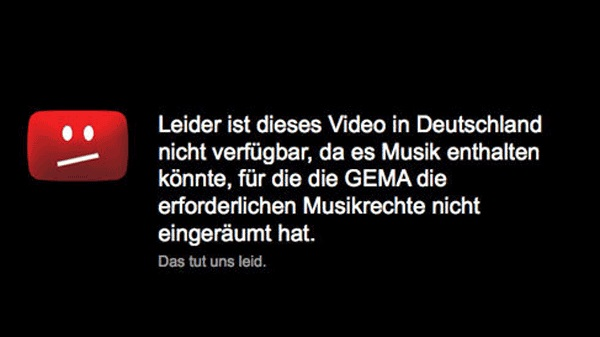
\includegraphics[scale=0.94]{se-wa-jpg/youtube_heise}
\caption[Rechtswidrige Sperrtafel von YouTube]{Rechtswidrige Sperrtafel von YouTube\protect\footnotemark}
\label{youtube_alt}
\end{figure}
\footnotetext{Vgl. Abbildung \textit{Briegleb}, Youtube-Hinweis wettbewerbswidrig, 2015.}

Nachdem Ablauf des Vertrages im März 2009 versuchten beide Parteien in zahlreichen Verhandlungen, einen Folgevertrag zu vereinbaren, was jedoch ohne Erfolg blieb. Resultierend aus den abgesprochenen Verhandlungsrunden im Mai 2010 entstanden die ersten Sperrtafeln, wie in \vref{youtube_alt} zu sehen. Dort heißt es von Seiten des Internet-Video-Diensts, dass \textit{die GEMA die erforderlichen Musikrechte nicht eingeräumt hat}. 

Von Seiten der GEMA hieß es: \glqq YouTube hat sich [...] entschieden, die von der
GEMA wahrgenommenen Rechte ohne jegliche Vergütung der Urheber zu nutzen – was aus Sicht
der GEMA einen Verstoß gegen das Urheberrecht darstellt.\grqq\seFootcite{}{S.1}{GEMA:YT} ~YouTube selbst sieht sich nur als ein \glqq Infrastruktur-Dienstleister\grqq, der seinen Nutzern eine Plattform zur Verfügung stellt, wodurch einige gerichtliche Verfahren entstanden sind und sogar bis heute laufen. Diese werden im Folgenden genauer aufgearbeitet.

\section{Gerichtliche Verfahren}		

Im Jahr 2010 erhebt die GEMA im Zusammenschluss mit sieben ausländischen Schwestergesellschaften eine \textbf{Unterlassungsklage} gegenüber YouTube vor dem Landgericht Hamburg, nachdem der Internet-Dienst für insgesamt 75 Werke, der Aufforderung des Löschens bzw. des Sperrens nicht nachkam. Dieser Antrag wurde jedoch aus formellen Gründen abgelehnt. Zwei Jahre später konnte YouTube jedoch für zehn ursprüngliche sowie zwei neu hinzugekommene Werke verurteilt werden. Grundlage dieses Rechtsspruch zur Unterlassung der Zugänglichmachung ist die \textit{Störerhaftung}, die besagt das YouTube die Prüfungs- und Kontrollpflichten verletzt und somit an der Rechtsverletzung des Urheberrechts mitwirkt. Der Konzern war daraufhin verpflichtet, alle Musikwerke auf illegale, öffentliche Nutzung zu prüfen. Mit den folgenden Mitteln geht YouTube dieser Verpflichtung nach:
\begin{itemize}
\item Einsatz eines MD5 und Content ID Filters
\item Einsatz eines Wortfilters
\item Warnhinweis an diejenigen Uploader, die versuchen, einen der bei YouTube als
rechtsverletzend bekannten Titel auf der Plattform einzustellen. 
\end{itemize}
Aus der Störerhaftung folglich muss YouTube die urheberrechtlich geschützten Videos entfernen, wenn Musiker, ggf. in Vertretung der GEMA, bei der Internetplattform Beschwerde einlegen.\seFootcite{Vgl.}{}{TS:G}
Da bis zum Ende der Berufungsfrist keine Einigung erzielt wurde, musste das Verfahren von dem Hanseatischen Oberlandesgericht in einer zweiten Instanz fortgeführt werden. Erst fünf Jahre nach der ersten Unterlassungsklage bestätigte das Oberlandesgericht das erstinstanzliche Urteil des Landgerichts Hamburg.\seFootcite{}{S.2}{GEMA:YT}

YouTube selbst streitet die urheberrechtliche Verantwortung der Inhalte ab und schiebt diese auf seine Nutzer, da die Werke nicht selbst von YouTube hochgeladen werden. Aus Sicht der GEMA jedoch bezieht YouTube durch seinen werbefinanzierten Streaming-Dienst einen wirtschaftlichen Vorteil, woraus eine Vergütung an die Künstler erfolgen sollte. Aus diesem Grund erfolgte am  10. Januar 2013 ein Antrag bei der Schiedsstelle des Deutschen Patent- und Markenamts, in deren Rahmen eine Überprüfung von über 1.000 urheberrechtlich geschützten Musikwerken des GEMA Repertoires gefordert wurde. Ziel der GEMA war eine angemessene Vergütung in Höhe von 0,375 Cent pro Stream (insgesamt rund 1,6 Millionen Euro), was jedoch in dem vorgeschriebenen Zeitrahmen nicht bearbeitet werden konnte und so das Verfahren ab dem 16. Mai 2014 vor dem ordentlichen Landgericht München fortgesetzt werden musste.\seFootcite{Vgl.}{}{R:ZO}

Das Landgericht München verkündete am 30. Juni 2015 das Urteil, wonach YouTube keiner \textbf{Schadensersatzzahlung} gegenüber der GEMA verpflichtet ist. Grundlage dafür sei, dass nicht YouTube selbst für den Upload der Werke verantwortlich sei, sondern die Nutzer. Aus Sicht des Gerichts sind also nur die Nutzer von YouTube selbst lizenzpflichtig. Auf der anderen Seite jedoch argumentiert die GEMA damit, dass YouTube durch die Werbeeinnahmen einen wirtschaftlichen Profit erzielt und sich dadurch eine Lizenzpflicht ergibt. Gegenüber dem Verfahren der Störhaftung ist in diesem Falle keine Verurteilung zum Schadensersatz möglich.\seFootcite{}{S.3}{GEMA:YT} Auch nachdem die GEMA Berufung gegen dieses Urteil eingelegt hatte, urteile im Januar 2016 auch das Oberlandesgericht München zugunsten des Internet-Dienstes. YouTube könne nicht wirtschaftlich zur Verantwortung gezogen werden, da die alleinige Verantwortung bei den Uploadern liegt. Dieses Urteil ist jedoch noch nicht rechtskräftig, da die GEMA Revision am Bundesgerichtshof eingeklagt hat.\seFootcite{Vgl.}{}{SD:G}

Im letzten großen Rechtsstreit zwischen GEMA und YouTube handelt es sich um die schon oben erwähnten \textbf{Sperrtafeln}. Seit Mitte 2011 schaltete YouTube - aus Sicht der GEMA willkürlich - sogenannte Sperrtafeln wie in \vref{youtube_alt} dargestellt. Mit dem Wortlaut \glqq Leider ist dieses Video in Deutschland nicht verfügbar, da es Musik enthalten könnte, für die die GEMA die erforderlichen Musikrechte nicht eingeräumt hat. Das tut  uns leid\grqq~versucht YouTube, die Schuld auf die Verwertungsgesellschaft zu schieben, so von Seiten der GEMA. Mit dieser \glqq irreführenden\grqq~ Sperrtafel würde der öffentliche Druck auf die GEMA erhöht werden, da ein falscher Eindruck entsteht.\seFootcite{Vgl.}{S.4}{GEMA:YT} Nachdem bereits im Februar 2014 in erster Instanz vom Landgericht München die Rechtswidrigkeit der Sperrtafeln festgestellt wurde, wurde auch am 7. Mai 2015 von Oberlandesgericht München die Schaltung der sogenannten \textit{GEMA-Sperrtafeln} als rechtswidrig eingestuft, was sogleich das erste Urteil zugunsten der Verwertungsgesellschaft war. Die Richter entschieden aufgrund der Tatsache, dass die GEMA irreführender Weise für die Sperrung von Inhalten verantwortlich sei, obwohl YouTube aus der Gesetzesgrundlage sowie dem Risiko des Störhafters die Videos selbst sperrt. Trotz des Einlegens einer Berufung gegen das Urteil seitens YouTube wurde das Urteil vom \gls{olg} als rechtskräftig gesprochen. Schon nach dem ersten Urteil wurde seit März 2014 die Sperrhinweise umformuliert. In \vref{youtube_neu} ist der neue Text zu sehen: \glqq Dieses Video ist in Deutschland leider nicht verfügbar, da es Musik enthalten könnte, über deren Verwendung wir uns mit der Gema bisher nicht einigen konnten. Das tut uns leid.\grqq\seFootcite{Vgl.}{}{SO:G}

\begin{figure}[H]
\centering
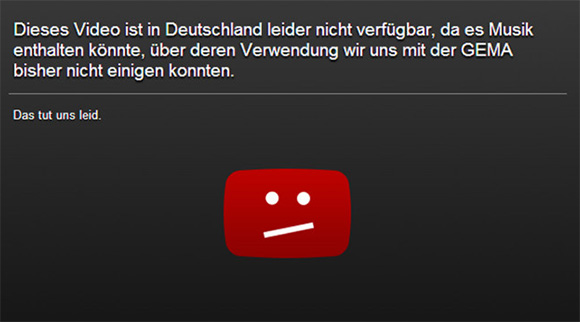
\includegraphics[scale=0.73]{se-wa-jpg/youtube_zeit}
\caption[Neue Sperrtafel von YouTube]{Neue Sperrtafel von YouTube\protect\footnotemark}
\label{youtube_neu}
\end{figure}
\footnotetext{Vgl. Abbildung \textit{Kühl}, YouTube neue Sperrtafel, 2014.}

\section{Heutiger Stand}
Nach fast zehn Jahren gerichtlicher Auseinandersetzungen laufen bis heute noch zwei Klageverfahren: Da wäre einmal die \textit{Klage auf Unterlassung}, die durch die Verurteilung YouTubes als Störhafter wenigstens einen kleinen Erfolg aufweisen konnte, andererseits gibt es noch das Verfahren der \textit{Klage auf Schadenersatz}, wobei die Summe des Schadenersatzes täglich durch neue Veröffentlichungen wächst.

Heiko Maas, der deutsche Bundesminister der Justiz und für Verbraucherschutz, brachte mit seiner Rede am 15. Januar 2016 vor dem Deutschen Bundestag neuen Schwung in die Debatte des Urheberrechts im Bezug auf die Rechte von Verwertungsgesellschaften. Ziel ist es, dem Anstoß aus Brüssel nachzukommen und die Rechte der Verwertungsgesellschaften europaweit harmonieren zu lassen. 50 Jahre wurde nach den Regeln der GEMA gespielt, nun soll das alte deutsche Urheberrechtswahrnehmungsgesetz abgelöst werden - im Mai 2016 wurde es schließlich außer Kraft gesetzt.\seFootcite{Vgl.}{S.1}{HM:NG} Maas' Rede stützt sich dabei auf die folgenden drei Punkte:

\begin{itemize}
\item Stärkere Mitbestimmung der Mitglieder in den Verwertungsgesellschaften
\item Anpassung des Rechts an das digitale Zeitalter (z.B. für Streamingangebote)
\item Reformation der Vergütung der Privatkopie, sodass Autoren und Verlage schneller an ihr Geld kommen
\end{itemize}

Gerade der zweite Punkt von Herrn Maas beinhaltet wichtige Überlegungen, die den Streit zwischen YouTube und GEMA endlich beenden könnten. Die Vergabe von den Musikrechten soll europaweit ausgeweitet werden, sodass nicht mehr mit der GEMA über die Urheberrechtsvergabe verhandelt werden muss.\seFootcite{Vgl.}{S.2}{HM:NG} Die bewährten Grundsätze sollen jedoch beibehalten werden. Die Verwertungsgesellschaften sollen weiterhin verpflichtet sein, die Nutzungsrechte zu angemessenen Bedingungen einzuräumen, wodurch der Wahrnehmungs- und Abschlusszwang erhalten bleibt. Weiterhin wird es die Aufgabe sein, Künstler zu unterstützen und zu fördern. 

Nachdem der Gesetzesentwurf bestätigt sowie anschließend am 28. April 2016 das Gesetz vom Bundestag beschlossen wurde, trat das neue \textbf{Verwertungsgesellschaftsgesetz} am 1. Juni 2016 in Kraft und löste damit das alte Urheberrechtswahrnehmungsgesetz ab. Wie in \vref{vgg} beschrieben, konnte somit ein europaweiter Mindeststandard im Bereich des Wahrnehmungsgesetzes erreicht werden. Ob dies endlich zu einer Einigung zwischen YouTube und der GEMA führt, bleibt weiterhin offen. Der Internet-Dienst könnte ja nun die erforderlichen Rechte europaweit erwerben - eine dafür vorgesehene Lizenzierungsstelle ist von der GEMA schon geplant. Letztlich wird durch das Gesetz auch die Mitbestimmung der Mitglieder einer Verwertungsgesellschaft gestärkt, sowie schon in Maas' Rede unter Punkt 1 angedacht.\seFootcite{Vgl.}{}{AP:G}
